\section{Global Cube Welding}
\label{sec:weld}

We first place every accepted cube mesh in volume coordinates and concatenate it under the ownership established by halo trimming. The uniformly coarse CVT interiors are desirable for scale, but their triangles are too large for the weld's ball of radius at most three voxels to initialize reliably. We therefore detect every internal cube plane and refine only a narrow seam band to approximately 3.5-voxel triangles (Fig.~\ref{fig:weld_bands}). Boundary half-edges in that band seed the same BPA used per cube, and four sub-processes then connect matching fronts while refusing invalid joins. A sliver cull first removes near-degenerate boundary triangles that would prime the bridge ball off a needle. The bridge front itself escalates its radius adaptively from the local boundary spacing, capped so that twice the maximum radius stays below the measured $\sim$7-voxel inter-wrap clearance --- welding two wraps together is therefore geometrically impossible for the bridge, not merely penalized. Every candidate bridge face must also pass a {\em winding gate}: its winding-phase gap $w = r/p - \theta/2\pi$ between front and candidate must stay within a soft tolerance (0.35 turns, with a 0.40-turn hard cap that separates legitimate grazing-seam closures from cross-layer and next-wrap stitches), which also keeps recto from welding to verso. Finally, a sheet-correspondence pass recovers legitimate same-sheet closures the conservative gate refused: it confirms a mutual-best 1:1 sheet pairing across each seam from bridge votes and boundary overlap, then re-welds only that confirmed pair on a point cloud restricted to those two sheets.

After each weld is complete, the temporary fine band is recoarsened and optimized with a {\em pinned-boundary} CVT/RVD pass. Boundary positions are held bit-exact while interior sites solve the same centroidal and normal-anisotropy objective as Section~\ref{sec:cvt}. A proposed band patch is accepted only if every pin is represented, the complete boundary-edge set is unchanged, all edges remain manifold, and both component count and Euler characteristic equal their pre-remesh values. Tiled passes with an offset allow long seams to be processed at bounded memory. If any invariant fails, that tile retains the pre-CVT weld.

We note that orientation consistency alone is insufficient to guarantee a valid scroll: a perfectly manifold bridge may still connect turns that are far apart in scroll phase. The global audit therefore measures abrupt full-turn edges and also computes a branch-local phase span, which detects broad fusions assembled from individually plausible edges. A phase sever can remove faces crossing those discontinuities, but its output remains unverified until every resulting component also satisfies the broad-span test. 

\begin{figure}[t]
  \centering
  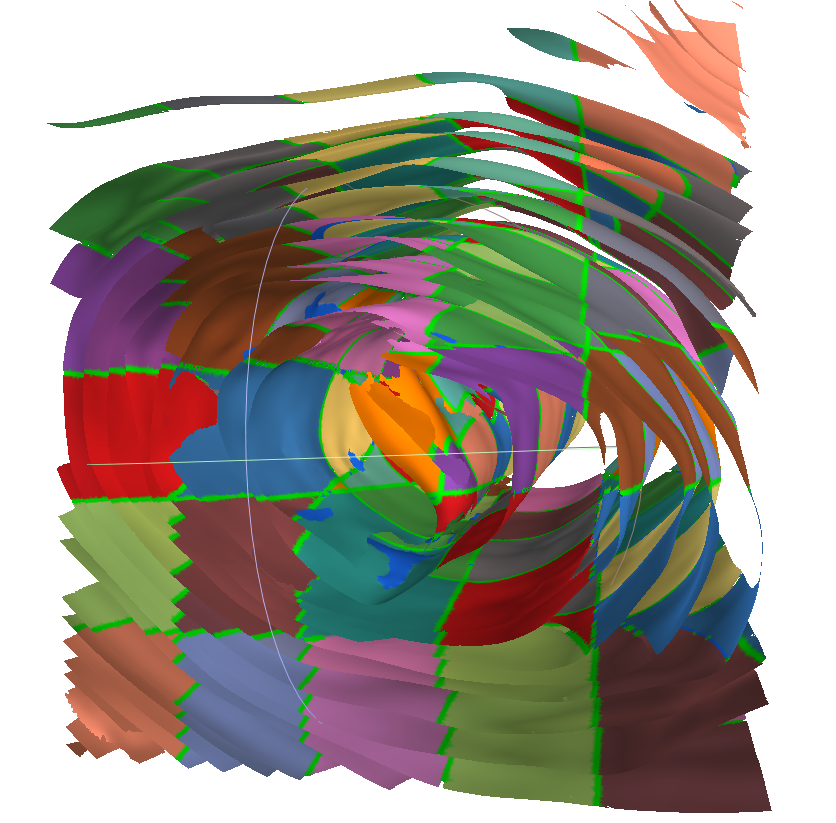
\includegraphics[width=\linewidth]{figures/welded_cube_4x5x5.png}
  \caption{The welded $4\times5\times5$ block with each cube's sheet coloured independently and the refined seam bands drawn in green. The weld bridges the $\sim$1-voxel trim gap between adjacent cubes only inside these bands; the winding gate and the capped bridge radius decide which fronts may join, so a sheet continues across a seam exactly when the two cubes agree it is the same wrap.}
  \Description{A rendered stack of curved papyrus sheets divided into cube-sized coloured tiles, with thin green bands marking the welded cube boundaries.}
  \label{fig:weld_bands}
\end{figure}

This weld is designed to compose hierarchically: a group of placed cubes or previously welded blocks enters the same seam-band procedure. The current complete validation is a flat $4\times5\times5$ block; the long $4\times21\times21$ experiment is decomposed into axial strips at the atlas level while the fully hierarchical geometry weld remains active work. In particular, our unwrapping and parameterization stage does not require the full weld, but uses it as a sub-engine to determine whether two sheets next to each other in UV space are in fact valid neighbours in the scroll itself.
